\documentclass{article}
\usepackage[utf8]{inputenc}
\usepackage{Preambles/preamble}

%~~~~~~~~~~~~~~~~~~~~~~~~~~~~~~~~~~~~~~~~~~~~~~~~~~~~~~~~~~~~~~~~~~~~~~~~~~~~~~~~~~~~~~~~~~~~~~%
%%%%%%%%%%%%%%%%%%%%%%%%%%%%%%%%%%%%%%%%%%%%%%%%%%%%%%%%%%%%%%%%%%%%%%%%%%%%%%%%%%%%%%%%%%%%%%%%
%                                                                                              % 
%             Template produced by Fergus Babb of the University of Nottingham, 2024           %
%                                                                                              %  
%%%%%%%%%%%%%%%%%%%%%%%%%%%%%%%%%%%%%%%%%%%%%%%%%%%%%%%%%%%%%%%%%%%%%%%%%%%%%%%%%%%%%%%%%%%%%%%%
%~~~~~~~~~~~~~~~~~~~~~~~~~~~~~~~~~~~~~~~~~~~~~~~~~~~~~~~~~~~~~~~~~~~~~~~~~~~~~~~~~~~~~~~~~~~~~~%

\begin{document}

%%%%%%%%%%%%%%%%%%%%%%%%%%%%%%%%%%%%%%%%%%%%%%%%%%%%%%%%%%%%%%%%%%%%%%%%%%%%%%%%%%%%%%%%%%%%%%%%
\title{Dynamic Parallel Maintaince of Strongly Connected Components in MPI}
%This isn't supposed to be for level of authorship, alphabetical is fine
\firstauthor{Soham Tripathy}
\firstID{CS20B073}
\firstemail{cs20b073@smail.iitm.ac.in}
\secondauthor{Name 2}
\secondID{Number ID 2}
\secondemail{ppyzzz@nottingham.ac.uk}
\supervisor{Professor. Rupesh Nasre}
\submitdate{\today}
\maketitle

\addtocounter{page}{-1}
\pagenumbering{roman}
\thispagestyle{empty}
%%%%%%%%%%%%%%%%%%%%%%%%%%%%%%%%%%%%%%%%%%%%%%%%%%%%%%%%%%%%%%%%%%%%%%%%%%%%%%%%%%%%%%%%%%%%%%%%

\newpage
\null\vspace{2in}
\begin{abstract}
This report explores the criticality of maintaining strongly connected components (SCCs) amidst dynamic changes in graph structures,
 emphasizing the efficiency of preserving SCCs during edge deletions and additions. Understanding the significance of SCCs in various applications,
 it becomes very challenging to recompute SCCs in response to changes in the graph structure. This requires efficient algorithms and optimization techniques
 to minimize the computational overhead and ensure real-time updates.
 Building upon prior research, we worked on extending an optimal algorithm tailored for this purpose. 
 The algorithm maintains the structure of strongly connnected components over sequence of edge updates in $O(mn)$ total time, with constant query time.
 This is an advancement over the best currently known deterministic algorithms, which run in $O(m^2)$ or $O(n^3)$ total time.
 Each facet of the algorithm deals with various cases of graph updates, which is elucidated with illustrative examples and accompanying pseudo code.
 
\vspace {1em}

Leveraging MPI for distributed parallel computation, we implement our algorithm,
 addressing encountered challenges and intricacies of the implementation process to facilitate comprehension of the code. 
 Detailed explanations of the design implementation, including the SCC tree construction, decremental and incremental maintenance, are provided.
 Rigorous testing on standard and specialized graphs, augmented with dynamic updates, is conducted, juxtaposing the performance against static SCC algorithms. 
 Results that are depicted through graphs and tables, are analyzed in the conclusion, offering insights and proposing avenues for future enhancements.
\end{abstract}
\vspace{\fill}
\thispagestyle{empty}

%~~~~~~~~~~~~~~~~~~~~~~~~~~~~~~~~~~~~~~~~~~~~~~~~~~~~~~~~~~~~~~~~~~~~~~~~~~~~~~~~~~~~~~~~~~~~~~~

\newpage
\doublespacing
\tableofcontents
\singlespacing

%~~~~~~~~~~~~~~~~~~~~~~~~~~~~~~~~~~~~~~~~~~~~~~~~~~~~~~~~~~~~~~~~~~~~~~~~~~~~~~~~~~~~~~~~~~~~~~~
%Sections before Main Content of report

\newpage

\section*{Acronyms}\label{Acronyms}
\addcontentsline{toc}{subsection}{\textit{Acronyms}}
\begin{description}[style=unboxed,font=\small]
    \item[MPI:]\label{mpi} Message Passing Interface
    \item[SCC:]\label{scc} Strongly Connected Components
    \item[STN:]\label{stn} SCC-Tree Node
  \end{description}
\vspace{2em}

\listoffigures
\addcontentsline{toc}{subsection}{\textit{List of Figures}}
\vspace{2em}

\listoftables
\addcontentsline{toc}{subsection}{\textit{List of Tables}}
\vspace{2em}
\newpage
\null\vspace{2in}
\section*{Acknowledgements}\label{Acknowledgements}
\addcontentsline{toc}{subsection}{\textit{Acknowledgements}}
\vspace{2em}
I would like to express my heartfelt gratitude to \emph{Professor Rupesh Nasre}, Department of Computer Science and Engineering, Indian Institute of Technology, Madras for his invaluable guidance,
 unwavering support, and insightful feedback throughout the duration of this project. 
 His expertise and mentorship have been instrumental in shaping the direction of this work.

\vspace {1em}

 Additionally, I extend my sincere appreciation to the M.Tech students, \emph{Barenya Kumar Nandy} and \emph{Anurag Sao}, whose valuable insights, 
 references, and constant assistance have greatly enriched this endeavor.

\vspace {1em}

I would also like to thank the Indian Institute of Technology, Madras, for providing the necessary resources and infrastructure for the successful completion of this project.

\vspace{2em}

\hfill Soham Tripathy
\vspace{\fill}

%~~~~~~~~~~~~~~~~~~~~~~~~~~~~~~~~~~~~~~~~~~~~~~~~~~~~~~~~~~~~~~~~~~~~~~~~~~~~~~~~~~~~~~~~~~~~~~~
%Main Content sections start

\newpage
\pagenumbering{arabic}
\section*{Main Content}%So pdf viewers dont have everything as a subsection of preamble
\addcontentsline{toc}{part}{Main Content}


\section{Introduction} \label{Sec: Introduction}
\blindtext
\cite[1]{Example_Reference}
\section{Literature Review} \label{Sec: Literature Review}
\blindtext
\section{Theoretical Methodology}\label{Sec: Theoretical Methodology}
In this part, we elaborate on and enhance the algorithm proposed in \cite{scc_tree_reference}
for maintaining strongly connected components (SCCs) under a sequence of updates. 
The algorithm is designed to accommodate n vertices and m edges as input, proficiently manages the following operations:
\begin{itemize}
 \item  \textsc{Query}(u, v): Verifies whether both u and v belong to the same SCC.
 \item  \textsc{Delete}(u, v): Removes the edge from u to v.
\item  \textsc{Add}(u, v): Introduces the edge from u to v.
\end{itemize}

This algorithm achieves its objectives through the creation and continuous maintenance of a specialized data structure known as the SCC Tree, 
which is further explained in the subsequent section. 
Additionally, it employs an SCC mapping array to facilitate queries in constant time \textit{O(1)}.

The algorithm initiates with an initialization stage, wherein it constructs the proposed SCC tree 
and populates the SCC mapping array based on the identified strongly connected components within the graph. 
Subsequently, the process of constructing and maintaining these pivotal data structures under the delete and add updates is elaborated in the following sections, accompanied by their respective pseudo codes.

\subsection{Data Structures}\label{Subsec: Data Structures Theoretical}

In this section, we delve into a comprehensive exploration of the specialized data structures crucial to the functionality 
and efficiency of the algorithm. Through this detailed examination, we aim to provide clarity 
and insight into the design principles, operational mechanisms, and computational complexities of these structures.

\subsubsection{SCC Tree}\label{Subsubsec: SCC Tree}
The \hyperref[scc]{SCC} tree serves as a vital component in maintaining the internal connectivity of vertices within the strongly connected components of graph G. 
For each SCC identified in the graph, a corresponding SCC tree is constructed.

The node in the SCC tree corresponding to the label $R$ encapsulates a tuple that can be represented as $\text{\textsc{STN}}(R) = \lf( V, E \rt)$, 
where $V$ represents set of vertices and $E$ represents set of edges connecting them. We can thus informally infer that \textsc{STN}(R) holds some graph-like structure $G$.
We will refer to the vertex set of the SCC tree node labeled $R$ as $\text{\textsc{STN}}(R).V$ and the edge set as $\text{\textsc{STN}}(R).E$.
This encapsulation enables the SCC tree to maintain the connectivity of the vertices that are a part of the SCC labeled $R$,
also facilitating efficient traversal and update operations.

Each vertex $v \in V$ in the \hyperref[stn]{STN} of $R$ is a label uniquely associated with an SCC tree. 
This tree is a subtree of the SCC tree represented by the label $R$.
The SCC tree for a graph containing one vertex $v$ has only a single \hyperref[stn]{STN} represented as $\text{\textsc{STN}}(v) = (\{v\}, \emptyset)$.

\begin{figure}[H]
    \centering
    \begin{subfigure}[b]{0.4\textwidth}
        \centering
        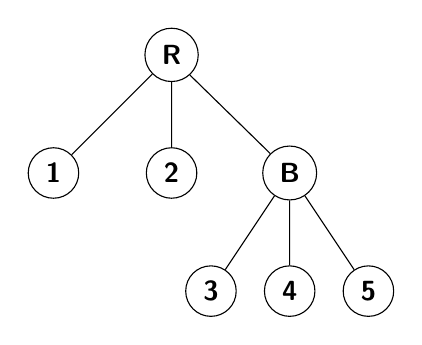
\begin{tikzpicture}[
            level distance=1.5cm,
            level 1/.style={sibling distance=1.5cm},
            level 2/.style={sibling distance=1cm},
            main node/.style={circle,draw,font=\sffamily\bfseries}]
                    % Define vertices
            \node[main node] (R) {R}
            child {node[main node] (1) {1}}
            child {node[main node] (2) {2}}
            child {node[main node] (B) {B}
                child {node[main node] (3) {3}}
                child {node[main node] (4) {4}}
                child {node[main node] (5) {5}}
            };
        \end{tikzpicture}
        \label{fig:example_scc_tree}
    \end{subfigure}
    \hfill
    \begin{subfigure}[b]{0.25\textwidth}
        \centering
        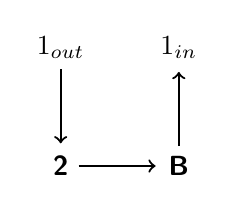
\begin{tikzpicture}[
            ->,shorten >=1pt,auto,node distance=1.5cm,
            thick,main node/.style={font=\sffamily\bfseries}]
            % Define vertices
        \node[main node] (1) {$1_{in}$};
        \node[main node] (11) [left of=1] {$1_{out}$};
        \node[main node] (2) [below of=11] {2};
        \node[main node] (B) [below of=1] {B};
        

        % Draw edges
        \path[every node/.style={font=\sffamily\small}]
            (11) edge (2)
            (2) edge (B)
            (B) edge (1);
        \end{tikzpicture}
        \caption{STN(R)}
        \label{fig:stn_r}
    \end{subfigure}
    \hfill 
    \begin{subfigure}[b]{0.25\textwidth}
        \centering
        \begin{tikzpicture}[
            ->,shorten >=1pt,auto,node distance=1.5cm,
            thick,main node/.style={font=\sffamily\bfseries}]
            % Define vertices
        \node[main node] (3) {$3_{in}$};
        \node[main node] (33) [left of=1] {$3_{out}$};
        \node[main node] (4) [below of=11] {4};
        \node[main node] (5) [below of=1] {5};
        

        % Draw edges
        \path[every node/.style={font=\sffamily\small}]
            (33) edge (4)
            (4) edge (5)
            (5) edge (3);
        \end{tikzpicture}
        \caption{STN(B)}
        \label{fig:stn_b}
    \end{subfigure}
    \caption{Example SCC Tree and its corresponding STNs}
    \label{fig:figure_with_subfigures}
\end{figure}

The SCC tree shown in \figureref{\ref{fig:figure_with_subfigures}}, can be represented by a collection of STNs as follows:
\begin{itemize}
    \item $\text{\textit{STN}}(R)=(\{1,2,B\}, \{(1,2), (2,B), (B,1)\})$
    \item $\text{\textit{STN}}(B)=(\{3,4,5\}, \{(3,4), (4,5), (5,3)\})$
    \item $\text{\textit{STN}}(v)=\lf(\{v\}, \emptyset\rt) \forall v \in \{1,2,3,4,5\}$
\end{itemize}
The SCC tree represented by label $B$ contains the STNs of $\{B,3,4,5\}$, which form a subtree of the SCC tree represented by label $R$,
similarly, the SCC tree represented by labels $\{1,2\}$ also form $R$'s subtree.

\subsubsection{SCC Mapping Array}\label{Subsubsec: SCC Mapping Array}
In graph G, each vertex $v$ is inherently associated with a strongly connected component (SCC), denoted by its corresponding SCC label. 
The SCC mapping array effectively captures this relationship between vertices and their respective SCC labels.

Suppose vertex $v$ in graph $G$ belongs to the strongly connected component labeled as $R$.
 In that case, we express this association using the SCC mapping array notation as $\text{\textsc{SM}}_{G}(v)=R$. 
 This signifies that vertex $v$ is mapped to the SCC labeled as $R$ within the context of the graph $G$.


\subsection{Definitions}\label{Subsec: Definitions Theoretical}
In this section, we establish key definitions that form the foundation of the algorithms presented subsequently. 
These definitions are instrumental in understanding the intricacies of the algorithms and their associated data structures.

\subsubsection{\textsc{FindScc}(G)}\label{Subsubsec: FindScc}
For a given graph $G$, let $V(G)$ represent the set of vertices of graph $G$.
We consider $k$ set of vertices as $U_i \forall i \in [1,k]$ such that it satisfies that following conditions:
\begin{itemize}
    \item $\bigcup\limits_{i=1}^{i=k}U_i = V(G)$
    \item $U_i \cap U_j = \emptyset$  $\forall i, j \in [1,k] | i \neq j$
    \item For each $U_i$, we say $\forall v, u \in U_i | v \neq u$, $\text{\textsc{Query}}(u, v) = true$.
    \item For any $U_i$ and $U_j$ such that $i \neq j$, $\forall v \in U_i$ and $\forall u \in U_j$, $\text{\textsc{Query}}(u, v) = false$.
\end{itemize}
We define the function \textsc{FindScc}(G) as the process of identifying the set of vertices $U_i$ that satisfies the above conditions.
The function \textsc{FindScc}(G) is instrumental in identifying the strongly connected components within the graph $G$.
We can do this by using any standard linear time algorithm, some of which are mentioned in \cite{find_scc_algorithm}, \cite{Kosaraju}, and \cite{DBLP:journals/corr/abs-2201-07197}.

\subsubsection{\textsc{Condense}(G)}\label{Subsubsec: Condense}

We define \textsc{Condense}(G) as condensing the graph $G$ into a new graph $G'$, where each vertex in $G'$ represents a strongly connected component in $G$,
$ie.$ $V(G') = \{\text{\textsc{SM}}_G(v) | v \in V(G)\}$.
The edges in $G'$ are such that if there is an edge from $u$ to $v$ in $G$, and $u$ and $v$ belong to different strongly connected components in $G$,
then there is an edge from the strongly connected component containing $u$ to the strongly connected component containing $v$ in $G'$. 
Therefore, a edge $(u, v) \in E(G) | \text{\textsc{Query}}(u, v) = false$ correponds to an edge $(\text{\textsc{SM}}_{G}(u), \text{\textsc{SM}}_{G}(v)) \in E(G')$.

\begin{algorithm}[H]
    \SetAlgoLined
    \KwData{G}
    \KwResult{G'}
    U = \text{\textsc{FindScc}}(G)\;
    \For {$U_i \in U$} {
        L = new label\;
        \For {$v \in U_i$} {
            $\text{\textsc{SM}}_G(v)$ = L\;
        }
        $V(G') = V(G')\cup L$
    }
    \For {$(u, v) \in E(G)$} {
        \If {$\text{\textsc{Query}}(u, v) = false$} {
            $E(G') = E(G') \cup (\text{\textsc{SM}}_G(u), \text{\textsc{SM}}_G(v))$
        }
    }
    \caption{\textsc{Condense}(G)}
\end{algorithm}

\subsubsection{\textsc{Split}(G,d)}\label{Subsubsec: Split}
Consider any graph G with a set of vertices $V(G)$ and a set of edges $E(G)$ such that $|\text{\textsc{FindScc}}(G)| = 1$.
Let $\exists d \in V(G)$ that can be split into two vertices $d_{in}$ and $d_{out}$ producing a new graph $G'$ 
such that any edge incident on $d$ is now incident on $d_{in}$ and any edge originating from $d$ is now originating from $d_{out}$.

\begin{algorithm}[H]
    \SetAlgoLined
    \KwData{G, d}
    \KwResult{G'}
    $V(G') = (V(G) \setminus \{d\}) \cup \{d_{in}, d_{out}\}$\;
    \For {$(u, v) \in E(G)$} {
        \If {$v = d$} {
            $E(G') = E(G') \cup (u, d_{in})$
        }
        \textbf{else} \If {$u = d$} {
            $E(G') = E(G') \cup (d_{out}, v)$
        }
        \Else {
            $E(G') = E(G') \cup (u, v)$
        }
    }
    \caption{\textsc{Split}(G,d)}
\end{algorithm}

\subsubsection{\textsc{Merge}(G, s, t, d)}\label{Subsubsec: Merge}
Let there be a graph $G$ such that it has a source vertex $s$ and a sink vertex $t$.
We define \textsc{Merge}(G,s,t, d) as merging the vertices $s$ and $t$ into vertex $d$ in the graph $G$ to produce a new graph $G'$.
This operation is the inverse of the \textsc{Split}(G, d) operation.

\begin{algorithm}[H]
    \SetAlgoLined
    \KwData{G,s,t,d}
    \KwResult{G'}
    $V(G') = V(G) \setminus \{t, s\} \cup \{d\}$\;
    \For {$(u, v) \in E(G)$} {
        \If {$v = t$} {
            $E(G') = E(G') \cup (u, d)$
        }
        \textbf{else} \If {$u = s$} {
            $E(G') = E(G') \cup (d, v)$
        }
        \Else {
            $E(G') = E(G') \cup (u, v)$
        }
    }
    \caption{\textsc{Merge}(G,s,t,d)}
\end{algorithm}

\subsubsection{\textsc{Unreachable}(G,s,t)}\label{Subsubsec: Unreachable}

Let there be a graph $G$ such that it has a source vertex $s$ and a sink vertex $t$.
A vertex $v$ is said to reachable if there exists a path from $s$ to $v$ and a path from $v$ to $t$.
We define the function \textsc{Unreachable}(G,s,t) as the process of identifying the set of vertices that are unreachable in $G$.

\begin{algorithm}[H]
    \SetAlgoLined
    \KwData{G, s, t}
    \KwResult{U}
    $U = \emptyset$\;
    $G' =$ \textsc{Merge}(G, s, t, d)\;
    $S = \text{\textsc{FindScc}}(G')$\;
    $R = \emptyset$\;
    \For {$U_i \in S$} {
        \If {$s \in U_i$} {
            $R = U_i$
        }
    }
    $U = V(G) \setminus R$\;
    \caption{\textsc{Unreachable}(G,s,t)}
\end{algorithm}


% subsection of construction of scc tree
\subsection{Constructing SCC Tree}

We will look at the construction of the SCC tree for the graph shown in \figureref{\ref{fig:graph1}}.
We start by finding all the SCCs of the graph and then construct the SCC-Tree for each SCC in it.
In the process of finding all the SCCs, we would also fill the SCC mapping array. 
A special tree node \textsc{STN}(M), called the master node would preserve the connectivity of the SCCs (condesed form of the original graph).
Suppose we have a strongly connected graph $G$, the SCC Tree for the graph is constructed as follows:
\begin{itemize}
    \item If $|V(G)| = 1$ and $v \in V(G)$, then the SCC tree is $SCC(v) = STN(v) = (\{v\}, \emptyset)$.
    \item If $|V(G)| > 1$ and $d \in V(G)$, then SCC-tree node would contain the graph \textsc{Condense}(\textsc{Split}($G, d$)), 
    and for each SCC in the graph \textsc{Condense}(\textsc{Split}($G, d$)), we add its SCC-tree as a subtree of R, with 
    exception that we would add only one tree for vertex $d$ instead of $d_{in}$ and $d_{out}$.
\end{itemize}

\begin{algorithm}
    \SetAlgoLined
    \KwData{G}
    \KwResult{SCC mapping, \textsc{SccTree}s, \textsc{STN}(M)}
    $SM_{G} = \emptyset, \textsc{SccTree} = \emptyset$\;
    $S = \textsc{FindSccs}(G), V_l = \emptyset, E_l = E(G)$\;
    \For {each $s \in S$} {
        $L_s = \textsc{Label}(s)$\;
        $G_s = G \cap s$\;
        $\textsc{SccTree}(L_s) = \textsc{MakeTree}(G_s, L_s)$\;
        \For {each $v \in s$} {
            $SM_{G}(v) = L_s$\;
        }
        $V_l = V \cup \{L_s\}$\;
        $E_l = E_l - \{e \in E(G_s)\}$\;
    }
    $\textsc{STN}(M) = (V_l, E_l)$\;
    \Return $SM_{G}, \textsc{SccTree}s, \textsc{STN}(M) = (V_l, E_l)$\;

    \caption{\textsc{ConstructDS}(G)}
\end{algorithm}

\begin{figure}[H]
    \centering
    \begin{subfigure}{0.45\textwidth}
        \centering
        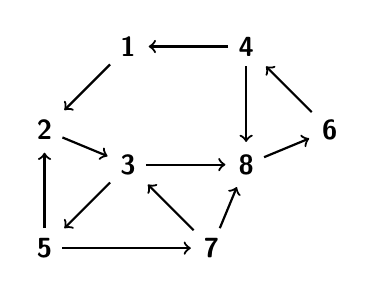
\begin{tikzpicture}[->,shorten >=1pt,auto,node distance=1.5cm,
            thick,main node/.style={font=\sffamily\bfseries}]

        % Define vertices
        \node[main node] (1) {1};
        \node[main node] (2) [below left of=1] {2};
        \node[main node] (3) [below of=1] {3};
        \node[main node] (4) [right of=1] {4};
        \node[main node] (5) [below left of=3] {5};
        \node[main node] (6) [below right of=4] {6};
        \node[main node] (7) [below right of=3] {7};
        \node[main node] (8) [right of=3] {8};
        

        % Draw edges
        \path[every node/.style={font=\sffamily\small}]
            (1) edge (2)
            (2) edge (3)
            (3) edge (5)
            (3) edge (8)
            (4) edge (1)
            (4) edge (8)
            (5) edge (2)
            (5) edge (7)
            (6) edge (4)
            (7) edge (3)
            (7) edge (8)
            (8) edge (6);

        \end{tikzpicture}
        \caption{Graph 1}
        \label{fig:graph1}
    \end{subfigure}
    \hfill
    \begin{subfigure}{0.45\textwidth}
        \centering
        
\begin{tikzpicture}[->,shorten >=1pt,auto,node distance=2cm,
            thick,main node/.style={circle,draw,font=\sffamily\bfseries}]

        % Define vertices
        \node[main node] (R) {R};

        \end{tikzpicture}
        \caption{condensed graph 1}
        \label{fig:condensed_graph1}
    \end{subfigure}
    \caption{Graph 1 and its condensed graph}
    \label{fig:graph1_and_condensed_graph1}
\end{figure}


%algorithm
\begin{algorithm}
    \SetAlgoLined
    \KwData{G | G is strongly connected, L | label of the root node}
    \KwResult{\textsc{SccTree(L)}}
    $v = random(V(G))$\;
    $\textsc{SccTree}(L) = \emptyset$\;
    \If {$|V(G)| = 1$} {
        $\textsc{STN}(L) = (\{v\}, \emptyset)$\;
        $\textsc{SccTree}(L) = \textsc{STN}(L)$\;
        \Return \textsc{SccTree}(L)\;
    }
    $G' = \textsc{Split}(G, v)$\;
    $S = \textsc{FindSccs}(G')$\;
    \For {each $s \in S$ and $v_{in} \not \in s$} {
        $L_s = \textsc{Label}(s)$\;
        $G_s = G' \cap s$\;
        $\textsc{SccTree}(L_s) = \textsc{MakeTree}(G_s, L_s)$\;
        $\textsc{SccTree}(L) = \textsc{SccTree}(L) \cup \textsc{SccTree}(L_s)$\;
    }
    $\textsc{STN}(L) = \textsc{Condense}(G')$\;
    $\textsc{SccTree}(L) = \textsc{SccTree}(L) \cup \textsc{STN}(L)$\;
    \Return \textsc{SccTree}(L)\;

    \caption{\textsc{MakeTree(G, L)}}
\end{algorithm}

We can understand the algorithm by looking at the following figures.
In \figureref{\ref{fig:graph1_and_condensed_graph1}}, we have the graph $G$, which is strongly connected.
Its condensed form would contain a single node $R$. The SCC mapping array would map all the nodes to $R$ and the master node 
would contain the graph in \figureref{\ref{fig:condensed_graph1}}.

After the strongly connected components of the graph are indentified, they are individually processed by the 
\textsc{MakeTree} algorithm. The algorithm starts by selecting a random vertex from the SCC and then splits the graph
on that vertex. The split graph is then condensed and the strongly connected components of the condensed graph are found. 
This is illustrated in \figureref{\ref{fig:scc_r_split_and_condensed_graph1}}, where we can see the condensed components $A$ and $B$.
The condesed graph in \figureref{\ref{fig:condensed_scc_r_split}} is stored in the \textsc{STN} of the root node $R$.
\begin{figure}[H]
    \centering
    \begin{subfigure}{0.45\textwidth}
        \centering
        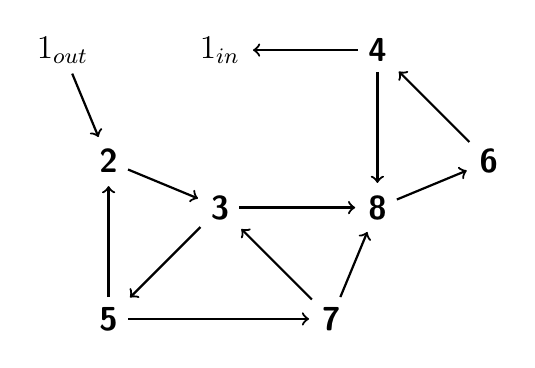
\begin{tikzpicture}[->,shorten >=1pt,auto,node distance=2cm,
            thick,main node/.style={font=\sffamily\large\bfseries}]

        % Define vertices
        \node[main node] (1) {$1_{in}$};
        \node[main node] (11) [left of=1] {$1_{out}$};
        \node[main node] (2) [below left of=1] {2};
        \node[main node] (3) [below of=1] {3};
        \node[main node] (4) [right of=1] {4};
        \node[main node] (5) [below left of=3] {5};
        \node[main node] (6) [below right of=4] {6};
        \node[main node] (7) [below right of=3] {7};
        \node[main node] (8) [right of=3] {8};
        

        % Draw edges
        \path[every node/.style={font=\sffamily\small}]
            (11) edge (2)
            (2) edge (3)
            (3) edge (5)
            (3) edge (8)
            (4) edge (1)
            (4) edge (8)
            (5) edge (2)
            (5) edge (7)
            (6) edge (4)
            (7) edge (3)
            (7) edge (8)
            (8) edge (6);

        \end{tikzpicture}
        \caption{SCC(R) split on 1}
        \label{fig:scc_r_split}
    \end{subfigure}
    \hfill
    \begin{subfigure}{0.45\textwidth}
        \centering
        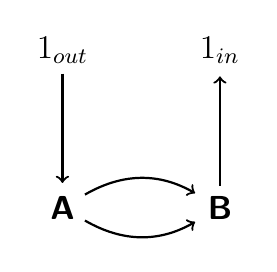
\begin{tikzpicture}[->,shorten >=1pt,auto,node distance=2cm,
            thick,main node/.style={font=\sffamily\large\bfseries}]

        % Define vertices
        \node[main node] (1) {$1_{in}$};
        \node[main node] (11) [left of=1] {$1_{out}$};
        \node[main node] (A) [below of=11] {A};
        \node[main node] (B) [below of=1] {B};
        

        % Draw edges
        \path[every node/.style={font=\sffamily\small}]
            (11) edge (A)
            (A) edge[bend left] (B)
            (A) edge[bend right] (B)
            (B) edge (1);

        \end{tikzpicture}
        \caption{condensed graph}
        \label{fig:condensed_scc_r_split}
    \end{subfigure}
    \caption{SCC(R) split on 1 and its condensed graph}
    \label{fig:scc_r_split_and_condensed_graph1}
\end{figure}

The \textsc{MakeTree} algorithm then processes all the condensed components of the split graph in a recursive manner.
The condensed component $A$ is split on 2, as in \figureref{\ref{fig:scc_a_split_and_condensed_graph1}}, and the 
condensed component $B$ is split on 4, as shown in \figureref{\ref{fig:scc_b_split_and_condensed_graph1}}. The 
component $A$ contains $C$ which is split on 3, as shown in \figureref{\ref{fig:scc_c_split_and_condensed_graph1}}.
The condesed graphs in \figureref{\ref{fig:condensed_scc_a_split}}, \figureref{\ref{fig:condensed_scc_b_split}}, and
\figureref{\ref{fig:condensed_scc_c_split}} are stored in the \textsc{STN} of $A$, $B$, and $C$ respectively.
\begin{figure}[H]
    \centering
    \begin{subfigure}{0.45\textwidth}
        \centering
        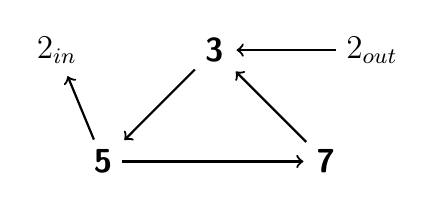
\begin{tikzpicture}[->,shorten >=1pt,auto,node distance=2cm,
            thick,main node/.style={font=\sffamily\large\bfseries}]

        % Define vertices
        \node[main node] (3) {3};
        \node[main node] (2) [right of=3] {$2_{out}$};
        \node[main node] (22) [left of=3] {$2_{in}$};
        \node[main node] (5) [below left of=3] {5};
        \node[main node] (7) [below right of=3] {7};
        

        % Draw edges
        \path[every node/.style={font=\sffamily\small}]
            (2) edge (3)
            (3) edge (5)
            (5) edge (22)
            (5) edge (7)
            (7) edge (3);

        \end{tikzpicture}
        \caption{SCC(A) split on 2}
        \label{fig:scc_a_split}
    \end{subfigure}
    \hfill
    \begin{subfigure}{0.45\textwidth}
        \centering
        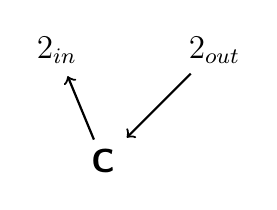
\begin{tikzpicture}[->,shorten >=1pt,auto,node distance=2cm,
            thick,main node/.style={font=\sffamily\large\bfseries}]

        % Define vertices
        \node[main node] (2) {$2_{out}$};
        \node[main node] (22) [left of=2] {$2_{in}$};
        \node[main node] (C) [below left of=2] {C};
        

        % Draw edges
        \path[every node/.style={font=\sffamily\small}]
            (2) edge (C)
            (C) edge (22);

        \end{tikzpicture}
        \caption{condensed graph}
        \label{fig:condensed_scc_a_split}
    \end{subfigure}
    \caption{SCC(A) split on 2 and its condensed graph}
    \label{fig:scc_a_split_and_condensed_graph1}
\end{figure}

\begin{figure}[H]
    \centering
    \begin{subfigure}{0.45\textwidth}
        \centering
        \begin{tikzpicture}[->,shorten >=1pt,auto,node distance=2cm,
            thick,main node/.style={font=\sffamily\large\bfseries}]

        % Define vertices
        \node[main node] (4) {$4_{in}$};
        \node[main node] (44) [left of=1] {$4_{out}$};
        \node[main node] (6) [below of=1] {6};
        \node[main node] (8) [below of=11] {8};
        

        % Draw edges
        \path[every node/.style={font=\sffamily\small}]
            (44) edge (8)
            (8) edge (6)
            (6) edge (4);

        \end{tikzpicture}
        \caption{SCC(B) split on 4}
        \label{fig:scc_b_split}
    \end{subfigure}
    \hfill
    \begin{subfigure}{0.45\textwidth}
        \centering
        \begin{tikzpicture}[->,shorten >=1pt,auto,node distance=2cm,
            thick,main node/.style={font=\sffamily\large\bfseries}]

        % Define vertices
        \node[main node] (4) {$4_{in}$};
        \node[main node] (44) [left of=1] {$4_{out}$};
        \node[main node] (6) [below of=1] {6};
        \node[main node] (8) [below of=11] {8};
        

        % Draw edges
        \path[every node/.style={font=\sffamily\small}]
            (44) edge (8)
            (8) edge (6)
            (6) edge (4);

        \end{tikzpicture}
        \caption{condensed graph}
        \label{fig:condensed_scc_b_split}
    \end{subfigure}
    \caption{SCC(B) split on 4 and its condensed graph}
    \label{fig:scc_b_split_and_condensed_graph1}
\end{figure}

\begin{figure}[H]
    \centering
    \begin{subfigure}{0.45\textwidth}
        \centering
        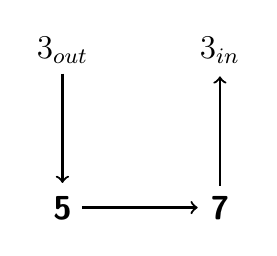
\begin{tikzpicture}[->,shorten >=1pt,auto,node distance=2cm,
            thick,main node/.style={font=\sffamily\large\bfseries}]

        % Define vertices
        \node[main node] (3) {$3_{in}$};
        \node[main node] (33) [left of=3] {$3_{out}$};
        \node[main node] (5) [below of=33] {5};
        \node[main node] (7) [below of=3] {7};
        

        % Draw edges
        \path[every node/.style={font=\sffamily\small}]
            (33) edge (5)
            (5) edge (7)
            (7) edge (3);

        \end{tikzpicture}
        \caption{SCC(C) split on 3}
        \label{fig:scc_c_split}
    \end{subfigure}
    \hfill
    \begin{subfigure}{0.45\textwidth}
        \centering
        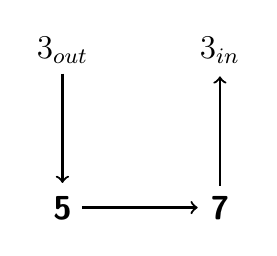
\begin{tikzpicture}[->,shorten >=1pt,auto,node distance=2cm,
            thick,main node/.style={font=\sffamily\large\bfseries}]

        % Define vertices
        \node[main node] (3) {$3_{in}$};
        \node[main node] (33) [left of=3] {$3_{out}$};
        \node[main node] (5) [below of=33] {5};
        \node[main node] (7) [below of=3] {7};
        

        % Draw edges
        \path[every node/.style={font=\sffamily\small}]
            (33) edge (5)
            (5) edge (7)
            (7) edge (3);

        \end{tikzpicture}
        \caption{condensed graph}
        \label{fig:condensed_scc_c_split}
    \end{subfigure}
    \caption{SCC(C) split on 3 and its condensed graph}
    \label{fig:scc_c_split_and_condensed_graph1}
\end{figure}

The figure \figureref{\ref{fig:scc_tree_graph1}} shows the SCC tree for the graph in \figureref{\ref{fig:graph1}}.
The SCC tree is constructed by the \textsc{MakeTree} algorithm, which recursively processes the condensed components of the split graph.
The child of each parent node in the SCC tree is a node present in the \textsc{STN} of the parent node.
\\$\textsc{SccTree(R)} = \textsc{STN}\text{'s of } \{R, 1, A, 2, C, 3, 5, 7, B, 4, 6, 8\}$


\begin{figure}[H]
    \centering
    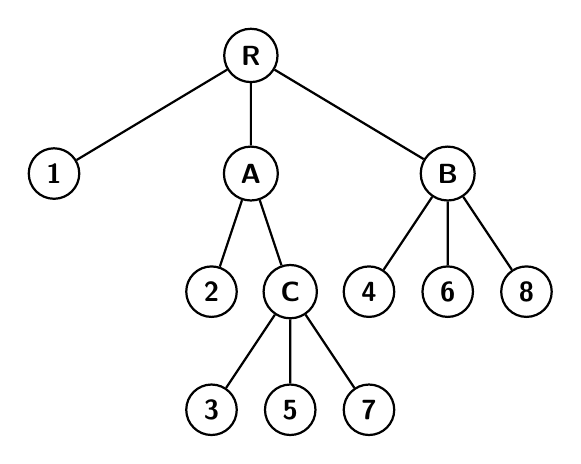
\begin{tikzpicture}[level distance=1.5cm,
                        level 1/.style={sibling distance=2.5cm},
                        level 2/.style={sibling distance=1cm},
                        thick,main node/.style={circle,draw,font=\sffamily\bfseries}]

      % Define vertices
      \node[main node] (R) {R}
        child {node[main node] (1) {1}}
        child {node[main node] (A) {A}
          child {node[main node] (2) {2}}
          child {node[main node] (C) {C}
            child {node[main node] (3) {3}}
            child {node[main node] (5) {5}}
            child {node[main node] (7) {7}}
          }
        }
        child {node[main node] (B) {B}
          child {node[main node] (4) {4}}
          child {node[main node] (6) {6}}
          child {node[main node] (8) {8}}
        };

    \end{tikzpicture}
    \caption{SCC Tree of Graph \ref{fig:graph1}}
    \label{fig:scc_tree_graph1}
\end{figure}



\subsection{Decremental Maintaince of SCC Tree}\label{Subsec: Decremental Maintaince of SCC Tree}

In this section, we delve into the decremental maintenance of the SCC tree under the delete operation.
As mentioned earlier, the \textsc{Delete}(u, v) operation removes the edge from vertex $u$ to vertex $v$ in the graph $G$.
This deletion operation necessitates the corresponding update in the SCC tree to maintain the internal connectivity of the vertices within the strongly connected components.
The deletion may also introduce new strongly connected components that may be formed due to the decomposition of the earlier SCCs.

Given, a graph $G$ and an edge $(u, v)$ is to be deleted from the graph $G$. Suppose if the vertex $u$ and $v$ belong to different strongly connected component, 
then the deletion of the edge $(u, v)$ will not affect any SCC tree. It would also not introduce any new SCCs, since the edge $(u, v)$ was not a part of any SCC.
In this case, we can simply remove the edge $(u, v)$ from the edge set of the master node.

However, if the vertices $u$ and $v$ belong to the same strongly connected component, then the deletion of the edge $(u, v)$ may introduce new SCCs or change the internal connectivity of the SCC tree.
Therefore, while we delete an edge $(u, v)$, we first must identify the SCC tree node that contains the edge $(u, v)$. This can be done by 
finding the lowest commen ancestor of the vertices $u$ and $v$ in the SCC tree. We then proceed to delete the edge from the identified node.

\begin{algorithm}[H]
    \SetAlgoLined
    \KwData{G, u, v}
    \KwResult{G'}
    \If {$\text{\textsc{Query}}(u, v) = false$} {
        $\text{\textsc{STN}}(M).E = \text{\textsc{STN}}(M).E \setminus \{(u, v)\}$\;
        \textbf{return}\;
    }
    $L = \text{\textsc{LCA}}(u, v)$\;
    $\text{\textsc{STN}}(L).E = \text{\textsc{STN}}(L).E \setminus \{(u, v)\}$\;
    \textsc{UpdateSCCTree}(L)\;
    \caption{\textsc{Delete}(G, u, v)}
\end{algorithm}

After the deletion of the edge $(u, v)$, we must ensure that the SCC tree is updated to reflect the changes in the internal connectivity of the vertices.
The updates ensures that the every vertex in each SCC tree node is reachable from the vertex $d_{out}$ and $d_{in}$, where $d$ is the vertex that was split to construct the SCC tree node,
we refer \secref{\ref{Subsubsec: Unreachable}} for the definition.

The following steps are performed to update the SCC tree after the deletion of the edge $(u, v)$ which belongs to the SCC tree node $L$, and $d$ is the vertex that was split to construct the SCC tree node $L$:
\begin{itemize}
    \item The unreachable vertices are removed form the SCC tree node $L$, and are added in the vertex set of the SCC tree node $p(L)$, where $p(L)$ denotes parent node of $L$.
If $L$ is the root node, then the unreachable vertices form new SCC-tree's, and thus updating the master node and the SCC mapping array.
    \item If vertices were removed from the SCC tree node $L$, then repeat the above steps for the parent node of $L$. This process stops when $L$ is the root node of the SCC tree, we then update the master node and the SCC mapping array.
    \item If unreachable vertices are present, then we expose the connectivity of these vertices to the parent node of $L$. This can be achieved by transferring
the edges that were a part of the unreachable vertices in $L$ to the parent node and also updating the edges in the edge set of the parent node that involved the unreachable vertices, which were a part of $L$.
This can be seen in \figureref{\ref{fig:tree_node_r_graph_exposed1}}, further details can be found in \secref{\ref{Subsubsec: Deleting Edge from the Root Node}} and \secref{\ref{Subsubsec: Deleting Edge from an Internal Node}}.
\end{itemize}

\begin{algorithm}[H]
    \SetAlgoLined
    \KwData{L | SCC Tree Node}
    \KwResult{Updated SCC Tree}
    $U = \text{\textsc{Unreachable}}(L, d_{in}, d_{out})$\;
    \textbf{if} {$U == \emptyset$} \textbf{then} \textbf{return}\;
    $E\_to\_expose = \emptyset$\;
    \hspace{1em}\\    \{Step 1: Removing vertices and edges\} \\
    \For {$v \in U$} {
        $\text{\textsc{STN}}(L).V = \text{\textsc{STN}}(L).V \setminus \{v\}$\;
    }
    \For {$(u, v) \in \text{\textsc{STN}}(L).E$} {
        \If {$u \in U$ or $v \in U$} {
            $\text{\textsc{STN}}(L).E = \text{\textsc{STN}}(L).E \setminus \{(u, v)\}$\;
            $E\_to\_expose = E\_to\_expose \cup \{(u, v)\}$\;
        }
    }
    \phantom{text}\\   \{Step 2: Exposing the connectivity\} \\
    \If {$L == \text{Root}$} {
        $p(L) = \textsc{STN}(M)$\;
    }
    \For {$(u, v) \in \textsc{STN}(p(L)).E$} {
        \For {$k \in U$} {
            $P = \textsc{SccTree}(k).Label$\;
            \If {$u \in P$} {
                $\textsc{STN}(p(L)).E = \textsc{STN}(p(L)).E \setminus \{(u, v)\}$\;
                $\textsc{STN}(p(L)).E = \textsc{STN}(p(L)).E \cup \{(k, v)\}$\;
            }
            \If {$v \in P$} {
                $\textsc{STN}(p(L)).E = \textsc{STN}(p(L)).E \setminus \{(u, v)\}$\;
                $\textsc{STN}(p(L)).E = \textsc{STN}(p(L)).E \cup \{(u, k)\}$\;
            }
        }
    }
    $\textsc{STN}(p(L)).E = \textsc{STN}(p(L)).E \cup E\_to\_expose$\;
    $\textsc{STN}(p(L)).V = \textsc{STN}(p(L)).V \cup U$\;
    \phantom{text}\\   \{ Step 3: Recursion (or) Updating the SCC Mapping Array\} \\
    \If {$L \neq \text{Root}$} {
        \textsc{UpdateSCCTree}(p(L))\;
    }
    \Else {
        \For {$v \in U$} {
            \For {$u \in \textsc{SccTree}(v).Label$} {
                \If {$\textsc{STN}(u).E == \emptyset$} {
                    $\textsc{SM}_G(u) = v$\;
                }
            }
        }
    }

    \caption{\textsc{UpdateSCCTree}(L)}
\end{algorithm}


\subsubsection{Deleting Edge from the Root Node}\label{Subsubsec: Deleting Edge from the Root Node}

\begin{figure}[H]
    \centering
    \begin{subfigure}{0.45\textwidth}
        \centering
        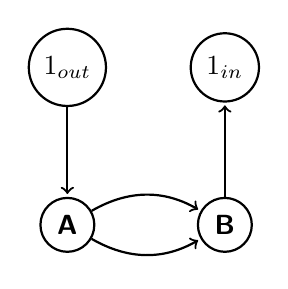
\begin{tikzpicture}[->,shorten >=1pt,auto,node distance=2cm,
            thick,main node/.style={circle,draw,font=\sffamily\bfseries}]

        % Define vertices
        \node[main node] (1) {$1_{in}$};
        \node[main node] (11) [left of=1] {$1_{out}$};
        \node[main node] (A) [below of=11] {A};
        \node[main node] (B) [below of=1] {B};
        

        % Draw edges
        \path[every node/.style={font=\sffamily\small}]
            (11) edge (A)
            (A) edge[bend left] (B)
            (A) edge[bend right] (B)
            (B) edge (1);

        \end{tikzpicture}
        \caption{Graph in SCC Tree Node R}
        \label{fig:tree_node_r_graph}
    \end{subfigure}
    \hfill
    \begin{subfigure}{0.45\textwidth}
        \centering
        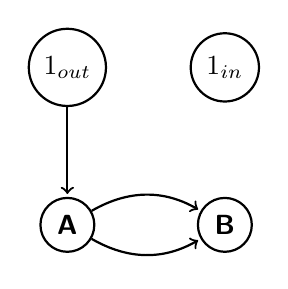
\begin{tikzpicture}[->,shorten >=1pt,auto,node distance=2cm,
            thick,main node/.style={circle,draw,font=\sffamily\bfseries}]

        % Define vertices
        \node[main node] (1) {$1_{in}$};
        \node[main node] (11) [left of=1] {$1_{out}$};
        \node[main node] (A) [below of=11] {A};
        \node[main node] (B) [below of=1] {B};
        

        % Draw edges
        \path[every node/.style={font=\sffamily\small}]
            (11) edge (A)
            (A) edge[bend left] (B)
            (A) edge[bend right] (B);

        \end{tikzpicture}
        \caption{Graph after deleting edge 4 to 1}
        \label{fig:graph_after_dedge_4_to_1}
    \end{subfigure}
    \caption{Graph in SCC Tree Node R after deleting edge 4 to 1}
    \label{fig:tree_node_r_graph_after_dedge1}
\end{figure}


\begin{figure}[H]
    \centering
    \begin{subfigure}{0.45\textwidth}
        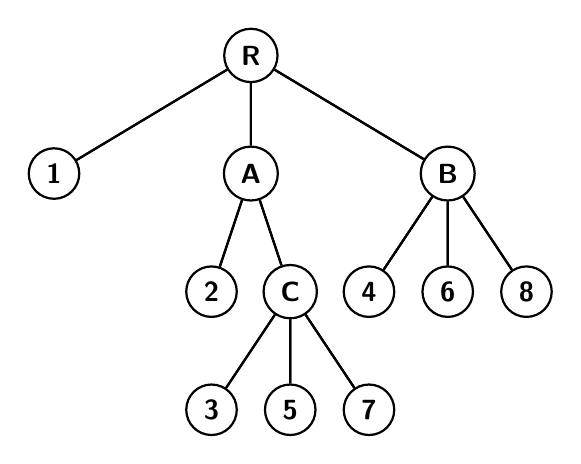
\begin{tikzpicture}[level distance=1.5cm,
                            level 1/.style={sibling distance=2.5cm},
                            level 2/.style={sibling distance=1cm},
                            thick,main node/.style={circle,draw,font=\sffamily\bfseries}]

        % Define vertices
        \node[main node] (R) {R}
            child {node[main node] (1) {1}}
            child {node[main node] (A) {A}
            child {node[main node] (2) {2}}
            child {node[main node] (C) {C}
                child {node[main node] (3) {3}}
                child {node[main node] (5) {5}}
                child {node[main node] (7) {7}}
            }
            }
            child {node[main node] (B) {B}
            child {node[main node] (4) {4}}
            child {node[main node] (6) {6}}
            child {node[main node] (8) {8}}
            };

        % Draw edges
        \path[every node/.style={font=\sffamily\small}]
            (R) edge (1)
            (R) edge (A)
            (R) edge (B)
            (A) edge (2)
            (A) edge (C)
            (B) edge (4)
            (B) edge (6)
            (B) edge (8)
            (C) edge (3)
            (C) edge (5)
            (C) edge (7);

        \end{tikzpicture}
        \caption{SCC Tree of Graph \ref{fig:graph1}}
        \label{fig:scc_tree_graph}
    \end{subfigure}
    \hfill
    \begin{subfigure}{0.5\textwidth}
        \centering
        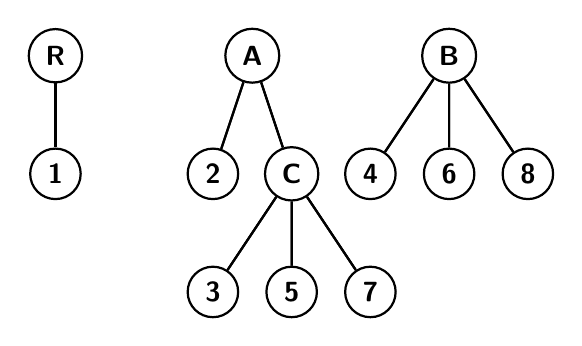
\begin{tikzpicture}[node distance=2.5cm,level distance=1.5cm,
                            level 1/.style={sibling distance=1cm},
                            level 2/.style={sibling distance=1cm},
                            thick,main node/.style={circle,draw,font=\sffamily\bfseries}]

        % Define vertices
        \node[main node] (R) {R}
            child {node[main node] (1) {1}};
        \node[main node] (A) [right of=R] {A}
            child {node[main node] (2) {2}}
            child {node[main node] (C) {C}
                child {node[main node] (3) {3}}
                child {node[main node] (5) {5}}
                child {node[main node] (7) {7}}
            };
        \node[main node] (B) [right of=A] {B}
            child {node[main node] (4) {4}}
            child {node[main node] (6) {6}}
            child {node[main node] (8) {8}};


        % Draw edges
        \path[every node/.style={font=\sffamily\small}]
            (R) edge (1)
            (A) edge (2)
            (A) edge (C)
            (B) edge (4)
            (B) edge (6)
            (B) edge (8)
            (C) edge (3)
            (C) edge (5)
            (C) edge (7);
        \end{tikzpicture}
        \caption{SCC Tree of Graph \ref{fig:graph1} after updates}
        \label{fig:scc_tree_graph_after_del}
    \end{subfigure}
    \caption{SCC Tree updates are propogated, deleting edge 4 to 1}
    \label{fig:scc_tree_after_update_propogation}
\end{figure}


\begin{figure}[H]
    \centering
    \begin{subfigure}{0.45\textwidth}
        \centering
        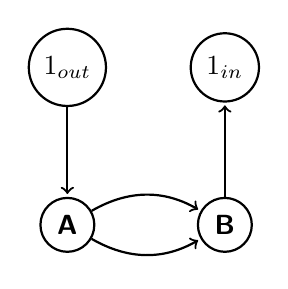
\begin{tikzpicture}[->,shorten >=1pt,auto,node distance=2cm,
            thick,main node/.style={circle,draw,font=\sffamily\bfseries}]

        % Define vertices
        \node[main node] (1) {$1_{in}$};
        \node[main node] (11) [left of=1] {$1_{out}$};
        \node[main node] (A) [below of=11] {A};
        \node[main node] (B) [below of=1] {B};
        

        % Draw edges
        \path[every node/.style={font=\sffamily\small}]
            (11) edge (A)
            (A) edge[bend left] (B)
            (A) edge[bend right] (B)
            (B) edge (1);

        \end{tikzpicture}
        \caption{Graph in SCC Tree Node R}
    \end{subfigure}
    \hfill
    \begin{subfigure}{0.45\textwidth}
        \centering
        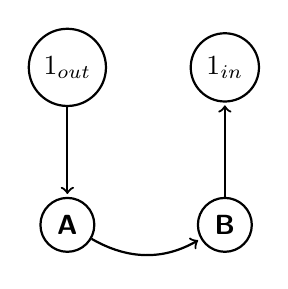
\begin{tikzpicture}[->,shorten >=1pt,auto,node distance=2cm,
            thick,main node/.style={circle,draw,font=\sffamily\bfseries}]

        % Define vertices
        \node[main node] (1) {$1_{in}$};
        \node[main node] (11) [left of=1] {$1_{out}$};
        \node[main node] (A) [below of=11] {A};
        \node[main node] (B) [below of=1] {B};
        

        % Draw edges
        \path[every node/.style={font=\sffamily\small}]
            (11) edge (A)
            (A) edge[bend right] (B)
            (B) edge (1);

        \end{tikzpicture}
        \caption{Graph after deleting edge 3 to 8}
        \label{fig:graph_after_dedge_3_to_8}
    \end{subfigure}
    \caption{Graph in SCC Tree Node R after deleting edge 3 to 8}
    \label{fig:tree_node_r_graph_after_dedge2}
\end{figure}
\subsubsection{Deleting Edge from an Internal Node}\label{Subsubsec: Deleting Edge from an Internal Node}

In this example, we consider the case when the deleted edge (u, v) belongs to an internal node of the SCC tree.
The edge (4, 8) is deleted from the graph held in \textsc{STN}(B), since the lowest common ancestor of 4 and 8 is B from the SCC tree in \figureref{\ref{fig:scc_tree_graph1}}.
We can see in \figureref{\ref{fig:tree_node_b_graph_after_dedge1}} that after removing the edge (4, 8) from the graph in \textsc{STN}(B), vertices 6 and 8 become unreachable from 4.


\begin{figure}[H]
    \centering
    \begin{subfigure}{0.45\textwidth}
        \centering
        \begin{tikzpicture}[->,shorten >=1pt,auto,node distance=2cm,
            thick,main node/.style={font=\sffamily\large\bfseries}]

        % Define vertices
        \node[main node] (4) {$4_{in}$};
        \node[main node] (44) [left of=1] {$4_{out}$};
        \node[main node] (6) [below of=1] {6};
        \node[main node] (8) [below of=11] {8};
        

        % Draw edges
        \path[every node/.style={font=\sffamily\small}]
            (44) edge (8)
            (8) edge (6)
            (6) edge (4);

        \end{tikzpicture}
        \caption{Graph in Tree Node B}
        \label{fig:tree_node_b_graph}
    \end{subfigure}
    \hfill
    \begin{subfigure}{0.45\textwidth}
        \centering
        \begin{tikzpicture}[->,shorten >=1pt,auto,node distance=2cm,
            thick,main node/.style={font=\sffamily\large\bfseries}]

        % Define vertices
        \node[main node] (4) {$4_{in}$};
        \node[main node] (44) [left of=1] {$4_{out}$};
        \node[main node] (6) [below of=1] {6};
        \node[main node] (8) [below of=11] {8};
        

        % Draw edges
        \path[every node/.style={font=\sffamily\small}]
            (8) edge (6)
            (6) edge (4);

        \end{tikzpicture}
        \caption{Graph after deleting edge 4 to 8}
        \label{fig:graph_after_dedge_4_to_8}
    \end{subfigure}
    \caption{Graph in Tree Node B after deleting edge 4 to 8}
    \label{fig:tree_node_b_graph_after_dedge1}
\end{figure}

Since, vertices 6 and 8 are unreachable from 4, we expose these vertices and the corresponding edges in \textsc{STN}(B) to its parent node R.
As shown in \figureref{\ref{fig:tree_node_r_graph_exposed1}}, the unreachable nodes 6 and 8 are exposed to the parent node R by adding edges (8,6), (6,4) from $B$ and
changing the edges (A,B), (B, $1_{in}$) in $R$ to (A,8), (4, $1_{in}$) respectively. The red line in \figureref{\ref{fig:tree_node_r_graph_exposed1}} shows the exposed graph
which was initially a part of $B$.

\begin{figure}[H]
    \centering
    \begin{subfigure}{0.45\textwidth}
        \centering
        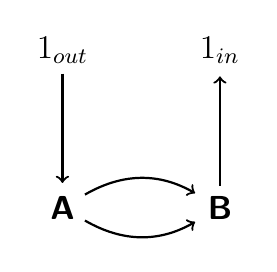
\begin{tikzpicture}[->,shorten >=1pt,auto,node distance=2cm,
            thick,main node/.style={font=\sffamily\large\bfseries}]

        % Define vertices
        \node[main node] (1) {$1_{in}$};
        \node[main node] (11) [left of=1] {$1_{out}$};
        \node[main node] (A) [below of=11] {A};
        \node[main node] (B) [below of=1] {B};
        

        % Draw edges
        \path[every node/.style={font=\sffamily\small}]
            (11) edge (A)
            (A) edge[bend left] (B)
            (A) edge[bend right] (B)
            (B) edge (1);

        \end{tikzpicture}
        \caption{Graph in SCC Tree Node R}
    \end{subfigure}
    \hfill
    \begin{subfigure}{0.45\textwidth}
        \centering
        \begin{tikzpicture}[->,shorten >=1pt,auto,node distance=2cm,
            thick,main node/.style={font=\sffamily\large\bfseries}]

        % Define vertices
        \node[main node] (1) {$1_{in}$};
        \node[main node] (11) [left of=1] {$1_{out}$};
        \node[main node] (A) [below left of=11] {A};
        \node[main node] (8) [below right of=A] {8};
        \node[main node] (6) [right of=8] {6};
        \node[main node] (4) [above right of=6] {4};
        

        % Draw edges
        \path[every node/.style={font=\sffamily\small}]
            (11) edge (A)
            (A) edge[bend left] (8)
            (A) edge[bend right] (8)
            (8) edge (6)
            (6) edge (4)
            (4) edge (1);

        \draw [red, rounded corners, dashed] ($(8) + (-0.5 , 0.5)$) -- ($(6) + (0,0.5)$) -- ($(4) + (-0.5, 0)$) -- ($(4) + (-0.5, 0.5)$) -- ($(4) + (0, 0.5)$) -- ($(4) + (0.5, 0.5)$) -- ($(4) + (0.5, 0)$) 
        -- ($(4) + (0.5, -0.25)$) -- ($(6) + (0.25, -0.5)$) -- ($(8) + (-0.5, -0.5)$) -- cycle;
        \end{tikzpicture}
        \caption{After Exposure}
        \label{fig:tree_node_r_graph_exposed1}
    \end{subfigure}
    \caption{Graph in SCC Tree Node R after unreachable nodes and its corresponding edges are exposed}
\end{figure}

We observe that every vertex in \figureref{\ref{fig:tree_node_r_graph_exposed1}} is reachable, thereby concluding the algorithm.
The above edge and vertex exposure process has a change in the SCC-tree, which is shown in \figureref{\ref{fig:scc_tree_after_update_propogation2}}.

\begin{figure}[H]
\centering
\begin{subfigure}{0.45\textwidth}
    \centering
    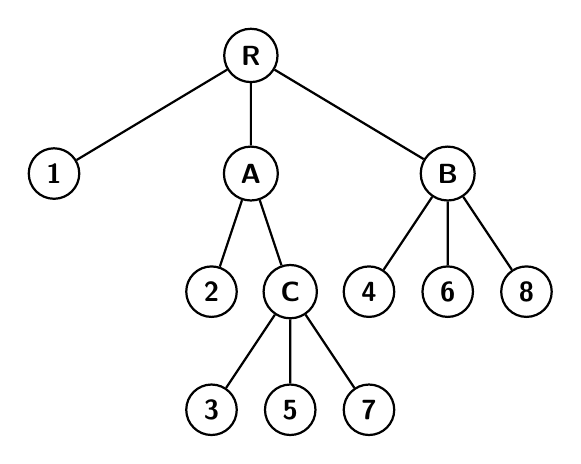
\begin{tikzpicture}[level distance=1.5cm,
                        level 1/.style={sibling distance=2.5cm},
                        level 2/.style={sibling distance=1cm},
                        thick,main node/.style={circle,draw,font=\sffamily\bfseries}]

    % Define vertices
    \node[main node] (R) {R}
        child {node[main node] (1) {1}}
        child {node[main node] (A) {A}
        child {node[main node] (2) {2}}
        child {node[main node] (C) {C}
            child {node[main node] (3) {3}}
            child {node[main node] (5) {5}}
            child {node[main node] (7) {7}}
        }
        }
        child {node[main node] (B) {B}
        child {node[main node] (4) {4}}
        child {node[main node] (6) {6}}
        child {node[main node] (8) {8}}
        };

    \end{tikzpicture}
    \caption{SCC Tree of Graph \ref{fig:graph1}}
\end{subfigure}
\hfill
\begin{subfigure}{0.45\textwidth}
    \centering
    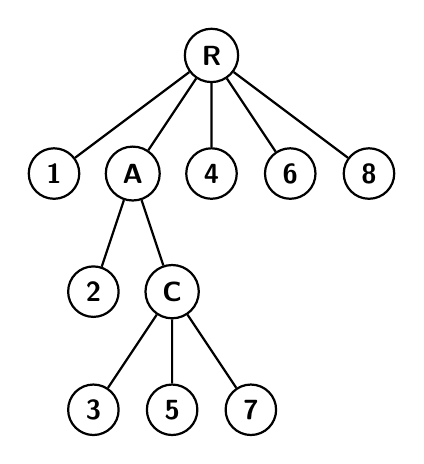
\begin{tikzpicture}[node distance=3cm,level distance=1.5cm,
                        level 1/.style={sibling distance=1cm},
                        level 2/.style={sibling distance=1cm},
                        thick,main node/.style={circle,draw,font=\sffamily\bfseries}]

    % Define vertices
    \node[main node] (R) {R}
        child {node[main node] (1) {1}}
        child {node[main node] (A) {A}
        child {node[main node] (2) {2}}
        child {node[main node] (C) {C}
        child {node[main node] (3) {3}}
        child {node[main node] (5) {5}}
        child {node[main node] (7) {7}}
        }
        }
        child {node[main node] (4) {4}}
        child {node[main node] (6) {6}}
        child {node[main node] (8) {8}}
        ;

    \end{tikzpicture}
    \caption{SCC Tree of Graph \ref{fig:graph1} after updates}
\end{subfigure}
\caption{Tree updates are propogated, deleting edge 4 to 8}
\label{fig:scc_tree_after_update_propogation2}
\end{figure}


\subsection{Incremental Maintaince of SCC Tree}\label{Subsec: Incremental Maintaince of SCC Tree}

In this section, we understand the process of maintaining the SCC tree under the add operation. The \textsc{Add}(u, v) operation introduces the edge from vertex $u$ to vertex $v$ in the graph $G$.
This operation when performed may join strongly connected components or change the internal connectivity of the SCC tree.

\begin{algorithm}[H]
    \SetAlgoLined
    \KwData{G, u, v}
    \KwResult{G'}
    $L = \text{\textsc{LCA}}(u, v)$\;
    $\text{\textsc{STN}}(L).E = \text{\textsc{STN}}(L).E \cup \{(u, v)\}$\;
    \textsc{UpdateSCCTreeI}(L)\;
    \caption{\textsc{Add}(G, u, v)}
\end{algorithm}

For graph $G$ and an edge $(u, v)$ is to be added to the graph $G$. Suppose if the vertex $u$ and $v$ belong to different strongly connected component, 
then the addition of the edge $(u, v)$ might combine multiple SCCs to form a sigle larger SCC. In this case, we add the edge $(u, v)$ to the master node
and update the SCC mapping array to reflect the newly formed SCC. A new SCC-tree node is introduced by adding the vertices and their corresponding edges which were a part of the SCCs that were combined in the master node.
These combined SCCs become the children of the newly formed SCC-tree node. This new SCC-tree node has to propogate its updates to maintain the internal connectivity of the vertices.

However, if the vertices $u$ and $v$ belong to the same strongly connected component, then the addition of the edge $(u, v)$ will never introduce any new SCCs, but would significantly change the internal structuring of the SCC tree.
These changes are to be propogated to maintain the SCC-tree structure and property.
The update propogation is nothing but re-running the SCC-tree creation algorithm on the SCC-tree node that has changes to propogate. The difference is that we do not have to re-run the algorithm on the entire graph, but only on the graphs stored in the SCC-tree nodes.

\begin{algorithm}[H]
    \SetAlgoLined
    \KwData{L | SCC Tree Node}
    \KwResult{Updated SCC Tree}
    $G = \textsc{STN}(L)$, $U = \text{\textsc{FindScc}}(G)$\;
    \For {$U_i \in U$ \textbf{and} $|U_i| \neq 1$} {
        $L_i = \textsc{Label}(U_i)$\;
        $\textsc{STN}(L_i) = \textsc{STN}(L) \cap U_i$\;
        $\textsc{STN}(L_i) = \textsc{Split}(\textsc{STN}(L_i), d)$\;
        $\textsc{UpdateSCCTreeI}(L_i)$\;
    }
    $\textsc{STN}(L) = \textsc{Condense}(G)$\;
    \For {$U_i \in U$ \textbf{and} $|U_i| = 1$} {
        $T = U_i$\;
        \While {$T \neq \emptyset$} {
            $V = T.pop()$\;
            \If {$\textsc{STN}(V).E == \emptyset$} {
                $\textsc{SM}_G(V) = L_i$\;
                \textbf{continue}\;
            }
            $T = T \cup \textsc{STN}(V).V$\;
        }
    }


    \caption{\textsc{UpdateSCCTreeI}(L)}
\end{algorithm}

\subsubsection{Updating SCC-tree under the Add operation}\label{Subsubsec: Updating SCC-tree under the Add operation}

We would now understand the process of updating the SCC-tree, when the edge $(u, v)$ is added to the graph $G$.
The graph in \figureref{\ref{fig:graph2}} is considered for this example, we can observe the SCC-tree of the graph in \figureref{\ref{fig:scc_tree2}}.
The graph has 3 stongly connected components which are identified by labels $R$, $5$ and $7$. 

\begin{figure}[H]
    \centering
    \begin{subfigure}{0.45\textwidth}
        \centering
        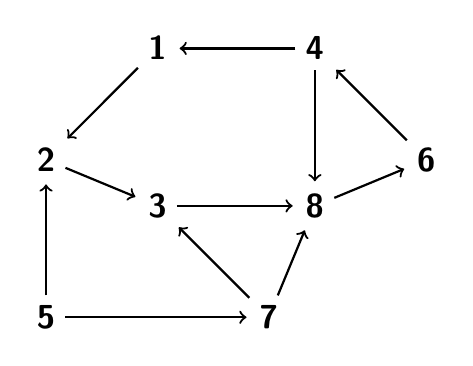
\begin{tikzpicture}[->,shorten >=1pt,auto,node distance=2cm,
                            thick,main node/.style={font=\sffamily\large\bfseries}]

        % Define vertices
        \node[main node] (1) {1};
        \node[main node] (2) [below left of=1] {2};
        \node[main node] (3) [below of=1] {3};
        \node[main node] (4) [right of=1] {4};
        \node[main node] (5) [below left of=3] {5};
        \node[main node] (6) [below right of=4] {6};
        \node[main node] (7) [below right of=3] {7};
        \node[main node] (8) [right of=3] {8};

        % Draw edges
        \path[every node/.style={font=\sffamily\small}]
            (1) edge (2)
            (2) edge (3)
            (3) edge (8)
            (4) edge (1)
            (4) edge (8)
            (5) edge (2)
            (5) edge (7)
            (6) edge (4)
            (7) edge (3)
            (7) edge (8)
            (8) edge (6);

        \end{tikzpicture}
        \caption{Graph 2}
        \label{fig:graph2}
    \end{subfigure}
    \begin{subfigure}{0.45\textwidth}
        \centering
        \begin{tikzpicture}[level distance=1.5cm,
                            level 1/.style={sibling distance=1.25cm},
                            level 2/.style={sibling distance=1cm},
                            thick,main node/.style={circle,draw,font=\sffamily\bfseries}]

        % Define vertices
        \node[main node] (R) {R}
            child {node[main node] (1) {1}}
            child {node[main node] (2) {2}}
            child {node[main node] (3) {3}}
            child {node[main node] (B) {B}
                child {node[main node] (4) {4}}
                child {node[main node] (6) {6}}
                child {node[main node] (8) {8}}
            };
        \node[main node, right=1.5cm of R] (5) {5};
        \node[main node, right=1.25cm of 5] (7) {7};
        \end{tikzpicture}

        \caption{SCC Tree of Graph 2} 
        \label{fig:scc_tree2}      
    \end{subfigure}
    \caption{Graph 2 and its SCC-trees}
    \label{fig:graph2_scc_tree}
\end{figure}
 

The edge $(3,5)$ is added to the graph, it combines the strongly connected components $R$, $5$ and $7$ to form a single SCC $R'$.
This change can be seen in the figure \figureref{\ref{fig:graph2_condense}}, we notice that the edge (3,5) correponds to the edge (R',5)
in the master node, which upon addtion combines the SCCs $R$, $5$ and $7$.

\begin{figure}[H]
    \centering
    \begin{subfigure}{0.4\textwidth}
        \centering
        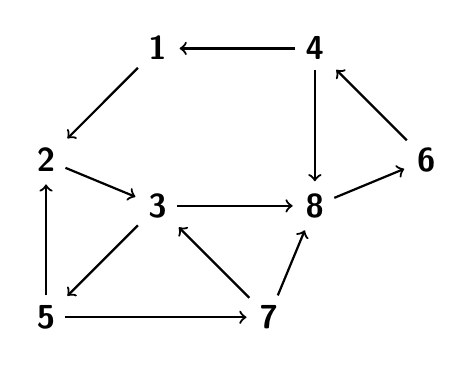
\begin{tikzpicture}[->,shorten >=1pt,auto,node distance=2cm,
                            thick,main node/.style={font=\sffamily\large\bfseries}]

        % Define vertices
        \node[main node] (1) {1};
        \node[main node] (2) [below left of=1] {2};
        \node[main node] (3) [below of=1] {3};
        \node[main node] (4) [right of=1] {4};
        \node[main node] (5) [below left of=3] {5};
        \node[main node] (6) [below right of=4] {6};
        \node[main node] (7) [below right of=3] {7};
        \node[main node] (8) [right of=3] {8};

        % Draw edges
        \path[every node/.style={font=\sffamily\small}]
            (1) edge (2)
            (2) edge (3)
            (3) edge (8)
            (4) edge (1)
            (4) edge (8)
            (5) edge (2)
            (5) edge (7)
            (6) edge (4)
            (7) edge (3)
            (7) edge (8)
            (8) edge (6)
            (3) edge (5);

        \end{tikzpicture}
        \caption{Graph 2}
    \end{subfigure}
    \begin{subfigure}{0.3\textwidth}
        \centering
        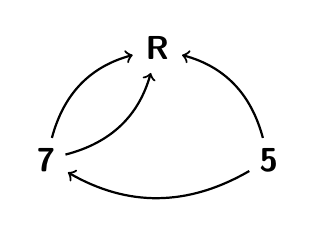
\begin{tikzpicture}[->,shorten >=1pt,auto,node distance=2cm,
                            thick,main node/.style={font=\sffamily\large\bfseries}]

        % Define vertices
        \node[main node] (R) {R};
        \node[main node] (5) [below right of=R] {5};
        \node[main node] (7) [below left of=R] {7};

        % Draw edges
        \path[every node/.style={font=\sffamily\small}]
            (5) edge[bend right] (R)
            (5) edge[bend left] (7)
            (7) edge[bend right] (R)
            (7) edge[bend left] (R);

        \end{tikzpicture}
        \caption{\textsc{Condense}(G) before \textsc{Add}}
        \label{fig:condense_before_add}      
    \end{subfigure}
    \begin{subfigure}{0.3\textwidth}
        \centering
        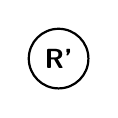
\begin{tikzpicture}[->,shorten >=1pt,auto,node distance=2cm,
                            thick,main node/.style={draw,circle,font=\sffamily\bfseries}]

        % Define vertices
        \node[main node] (R') {R'};

        \end{tikzpicture}
        \caption{\textsc{Condense}(G) after \textsc{Add}}
        \label{fig:condense_after_add}
    \end{subfigure}
    \caption{Graph 2, \textsc{Condense}(G) before and after \textsc{Add}}
    \label{fig:graph2_condense}
\end{figure}
 

A new SCC-tree node $R'$ is introduced to represent the new SCC formed by the addition of the edge $(3,5)$.
It captures the subgraph that is formed by the vertices and edges that were a part of the SCCs $R$, $5$ and $7$.
The SCC-tree node $R'$ graph is split on the vertex $7$, as shown in \figureref{\ref{fig:stn_r_before_after_split}}.
When we condense the graph in \textsc{STN}(R'), we find that the vertices $R$ and $5$ combine to form a single vertex $A$, as shown in \figureref{\ref{fig:stn_a_and_updated_scc_tree}}.

\begin{figure}[H]
    \centering
    \begin{subfigure}{0.3\textwidth}
        \centering
        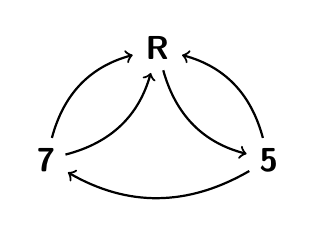
\begin{tikzpicture}[->,shorten >=1pt,auto,node distance=2cm,
                            thick,main node/.style={font=\sffamily\large\bfseries}]

        % Define vertices
        \node[main node] (R) {R};
        \node[main node] (5) [below right of=R] {5};
        \node[main node] (7) [below left of=R] {7};

        % Draw edges
        \path[every node/.style={font=\sffamily\small}]
            (5) edge[bend right] (R)
            (5) edge[bend left] (7)
            (7) edge[bend right] (R)
            (7) edge[bend left] (R)
            (R) edge[bend right] (5);

        \end{tikzpicture}
        \caption{\textsc{STN}(R') before \textsc{Split}}
    \end{subfigure}
    \begin{subfigure}{0.3\textwidth}
        \centering
        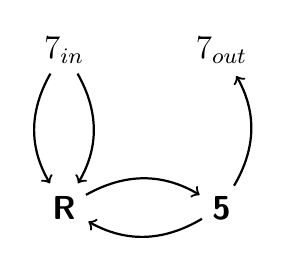
\begin{tikzpicture}[->,shorten >=1pt,auto,node distance=2cm,
                            thick,main node/.style={font=\sffamily\large\bfseries}]

        % Define vertices
        \node[main node] (7) {$7_{in}$};
        \node[main node] (77) [right of=7] {$7_{out}$};
        \node[main node] (5) [below of=77] {5};
        \node[main node] (R) [below of=7] {R};

        % Draw edges
        \path[every node/.style={font=\sffamily\small}]
            (7) edge[bend right] (R)
            (7) edge[bend left] (R)
            (5) edge[bend right] (77)
            (5) edge[bend left] (R)
            (R) edge[bend left] (5);

        \end{tikzpicture}
        \caption{\textsc{STN}(R') after \textsc{Split}}
    \end{subfigure}
    \begin{subfigure}{0.3\textwidth}
        \centering
        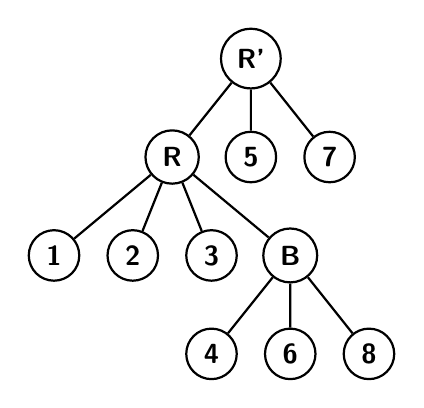
\begin{tikzpicture}[level distance=1.25cm,
                            level 1/.style={sibling distance=1cm},
                            level 2/.style={sibling distance=1cm},
                            thick,main node/.style={circle,draw,font=\sffamily\bfseries}]

        % Define vertices
        \node[main node] (R') {R'}
            child {node[main node] (R) {R}
                child {node[main node] (1) {1}}
                child {node[main node] (2) {2}}
                child {node[main node] (3) {3}}
                child {node[main node] (B) {B}
                    child {node[main node] (4) {4}}
                    child {node[main node] (6) {6}}
                    child {node[main node] (8) {8}}
                }
            }
            child {node[main node] (5) {5}}
            child {node[main node] (7) {7}};
        \end{tikzpicture}

        \caption{updated SCC-tree}     
    \end{subfigure}
    \caption{\textsc{STN}(R') before and after \textsc{Split} and updated SCC-tree}
    \label{fig:stn_r_before_after_split}
\end{figure}
 

The new SCC-tree node $A$ is introduced that captures the subgraph formed by the vertices and edges that were a part of $R$ and $5$, in the SCC-tree node $R'$. 
This graph can be seen in \figureref{\ref{fig:stn_a_and_updated_scc_tree}}, when we condense the graph in \textsc{STN}(A), we find that no combination of vertices is possible, and thus the SCC-tree is updated.
The SCC-tree is updated to reflect changes brought by the addition of the edge $(3,5)$ is shown in \figureref{\ref{fig:stn_a_and_updated_scc_tree}}.

\begin{figure}[H]
    \centering
    \begin{subfigure}{0.3\textwidth}
        \centering
        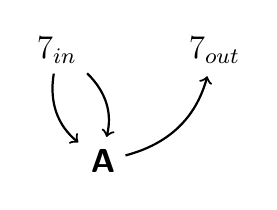
\begin{tikzpicture}[->,shorten >=1pt,auto,node distance=2cm,
                            thick,main node/.style={font=\sffamily\large\bfseries}]

        % Define vertices
        \node[main node] (7) {$7_{in}$};
        \node[main node] (77) [right of=7] {$7_{out}$};
        \node[main node] (A) [below left of=77] {A};

        % Draw edges
        \path[every node/.style={font=\sffamily\small}]
            (7) edge[bend right] (A)
            (7) edge[bend left] (A)
            (A) edge[bend right] (77);

        \end{tikzpicture}
        \caption{\textsc{STN}(R') after \textsc{Condense}}
    \end{subfigure}
    \begin{subfigure}{0.3\textwidth}
        \centering
        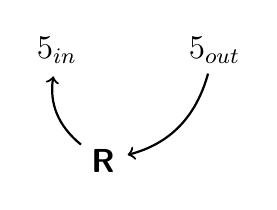
\begin{tikzpicture}[->,shorten >=1pt,auto,node distance=2cm,
                            thick,main node/.style={font=\sffamily\large\bfseries}]

        \node[main node] (5) {$5_{in}$};
        \node[main node] (55) [right of=5] {$5_{out}$};
        \node[main node] (R) [below left of=55] {R};

        \path[every node/.style={font=\sffamily\small}]
            (55) edge[bend left] (R)
            (R) edge[bend left] (5);

        \end{tikzpicture}
        \caption{\textsc{STN}(A)}
    \end{subfigure}
    \begin{subfigure}{0.3\textwidth}
        \centering
        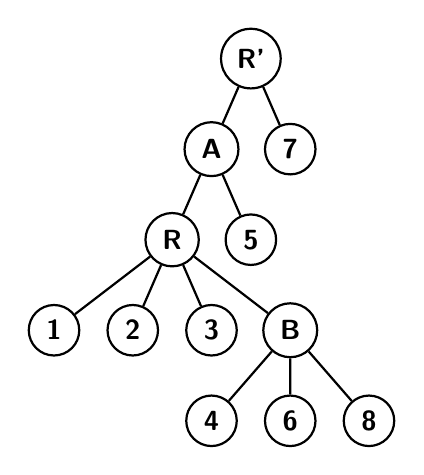
\begin{tikzpicture}[level distance=1.15cm,
                            level 1/.style={sibling distance=1cm},
                            level 2/.style={sibling distance=1cm},
                            thick,main node/.style={circle,draw,font=\sffamily\bfseries}]

        % Define vertices
        \node[main node] (R') {R'}
            child {node[main node] (A) {A}
                child {node[main node] (R) {R}
                    child {node[main node] (1) {1}}
                    child {node[main node] (2) {2}}
                    child {node[main node] (3) {3}}
                    child {node[main node] (B) {B}
                        child {node[main node] (4) {4}}
                        child {node[main node] (6) {6}}
                        child {node[main node] (8) {8}}
                    }
                }
                child {node[main node] (5) {5}}
            }
            child {node[main node] (7) {7}};
        \end{tikzpicture}

        \caption{updated SCC-tree}     
    \end{subfigure}
    \caption{\textsc{STN}(R'), \textsc{STN}(A) and updated SCC-tree}
    \label{fig:stn_a_and_updated_scc_tree}
\end{figure}
 



\section{Practical Implementation} \label{Sec: Practical Implementation}
\blindtext
\subsection{Data Structures}\label{Subsec: Data Structures}
\blindtext
\subsection{Workload Distribution in Parallel}\label{Subsec: Workload Distribution in Parallel}
\blindtext
\subsection{Update Cache Optimizations}\label{Subsec: Cache Optimizations}
\blindtext
\begin{table}[H]
    \centering
    \caption{Timings with/without Cache Optimizations}
    \begin{tabular}{|c|c|c|}
        \hline
        \textbf{Updates(\%)} & \textbf{With Caching} & \textbf{Without Caching} \\
        \hline
        \texttt{0} & 3,072,441 & 234,370,166 \\
        \texttt{1} & 58,655,849 & 261,321,071 \\
        \texttt{5} & 3,370,462 & 93,373,056 \\
        \texttt{10} & 4,847,571 & 68,993,773 \\
        \texttt{15} & 1,632,803 & 30,622,564 \\
        \texttt{20} & 21,297,772 & 265,025,809 \\
        \texttt{30} & 16,777,216 & 87,654,320 \\
        \texttt{50} & 10,000,000 & 80,000,000 \\
        \hline
    \end{tabular}
    \label{tab:cache_optimizations}
\end{table}

\subsection{Challenges in Implementation with MPI}\label{Subsec: Challenges in Implementation with MPI}
\blindtext



\section{Results}\label{Sec: Results}
\blindtext

\begin{table}[H]
    \centering
    \caption{Graph Details}
    \begin{tabular}{|c|c|c|}
        \hline
        \textbf{Graph} & \textbf{Number of Vertices} & \textbf{Number of Edges} \\
        \hline
        \texttt{cleancom-orkutud-SCC} & 3,072,441 & 234,370,166 \\
        \texttt{clean-soc-sinaweibo-SCC} & 58,655,849 & 261,321,071 \\
        \texttt{cleanWikipedia-SCC} & 3,370,462 & 93,373,056 \\
        \texttt{livjournal-SCC} & 4,847,571 & 68,993,773 \\
        \texttt{clean-soc-pokec-relationships-SCC} & 1,632,803 & 30,622,564 \\
        \texttt{clean-soc-twitter-SCC} & 21,297,772 & 265,025,809 \\
        \texttt{rmat876-SCC} & 16,777,216 & 87,654,320 \\
        \texttt{u10m\_80m-SCC} & 10,000,000 & 80,000,000 \\
        \hline
    \end{tabular}
    \label{tab:graph_details}
\end{table}


\begin{table}[H]
    \centering
    \caption{Timings for Graph \texttt{cleancom-orkutud-SCC} }
    \begin{tabular}{|c|c|c|c|c|c|c|}
        \hline
        \textbf{Update(\%)} & \multicolumn{2}{c|}{\textbf{Decremental}} & \multicolumn{2}{c|}{\textbf{Incremental}} & \multicolumn{2}{c|}{\textbf{Both}} \\
        \hline
        w.r.t. edges & Static &  Dynamic & Static & Dynamic & Static & Dynamic \\
        \hline
        0 & 1.0 & 1.1 & 1.2 & 1.3 & 1.4 & 1.5 \\
        1 & 2.3 & 2.4 & 2.5 & 2.6 & 2.7 & 2.8 \\
        5 & 2.9 & 3.0 & 3.1 & 3.2 & 3.3 & 3.4 \\
        10 & 3.5 & 3.6 & 3.7 & 3.8 & 3.9 & 4.0 \\
        15 & 4.1 & 4.2 & 4.3 & 4.4 & 4.5 & 4.6 \\
        20 & 4.1 & 4.2 & 4.3 & 4.4 & 4.5 & 4.6 \\
        30 & 4.7 & 4.8 & 4.9 & 5.0 & 5.1 & 5.2 \\
        \hline
    \end{tabular}
    \label{tab:timed_results_g1}
\end{table}

\begin{table}[H]
    \centering
    \caption{Timings for Graph \texttt{clean-soc-sinaweibo-SCC} }
    \begin{tabular}{|c|c|c|c|c|c|c|}
        \hline
        \textbf{Update(\%)} & \multicolumn{2}{c|}{\textbf{Decremental}} & \multicolumn{2}{c|}{\textbf{Incremental}} & \multicolumn{2}{c|}{\textbf{Both}} \\
        \hline
        w.r.t. edges & Static &  Dynamic & Static & Dynamic & Static & Dynamic \\
        \hline
        0 & 1.0 & 1.1 & 1.2 & 1.3 & 1.4 & 1.5 \\
        1 & 2.3 & 2.4 & 2.5 & 2.6 & 2.7 & 2.8 \\
        5 & 2.9 & 3.0 & 3.1 & 3.2 & 3.3 & 3.4 \\
        10 & 3.5 & 3.6 & 3.7 & 3.8 & 3.9 & 4.0 \\
        15 & 4.1 & 4.2 & 4.3 & 4.4 & 4.5 & 4.6 \\
        20 & 4.1 & 4.2 & 4.3 & 4.4 & 4.5 & 4.6 \\
        30 & 4.7 & 4.8 & 4.9 & 5.0 & 5.1 & 5.2 \\
        \hline
    \end{tabular}
    \label{tab:timed_results_g2}
\end{table}

\begin{table}[H]
    \centering
    \caption{Timings for Graph \texttt{cleanWikipedia-SCC} }
    \begin{tabular}{|c|c|c|c|c|c|c|}
        \hline
        \textbf{Update(\%)} & \multicolumn{2}{c|}{\textbf{Decremental}} & \multicolumn{2}{c|}{\textbf{Incremental}} & \multicolumn{2}{c|}{\textbf{Both}} \\
        \hline
        w.r.t. edges & Static &  Dynamic & Static & Dynamic & Static & Dynamic \\
        \hline
        0 & 1.0 & 1.1 & 1.2 & 1.3 & 1.4 & 1.5 \\
        1 & 2.3 & 2.4 & 2.5 & 2.6 & 2.7 & 2.8 \\
        5 & 2.9 & 3.0 & 3.1 & 3.2 & 3.3 & 3.4 \\
        10 & 3.5 & 3.6 & 3.7 & 3.8 & 3.9 & 4.0 \\
        15 & 4.1 & 4.2 & 4.3 & 4.4 & 4.5 & 4.6 \\
        20 & 4.1 & 4.2 & 4.3 & 4.4 & 4.5 & 4.6 \\
        30 & 4.7 & 4.8 & 4.9 & 5.0 & 5.1 & 5.2 \\
        \hline
    \end{tabular}
    \label{tab:timed_results_g3}
\end{table}


\begin{table}[H]
    \centering
    \caption{Timings for Graph \texttt{livjournal-SCC} }
    \begin{tabular}{|c|c|c|c|c|c|c|}
        \hline
        \textbf{Update(\%)} & \multicolumn{2}{c|}{\textbf{Decremental}} & \multicolumn{2}{c|}{\textbf{Incremental}} & \multicolumn{2}{c|}{\textbf{Both}} \\
        \hline
        w.r.t. edges & Static &  Dynamic & Static & Dynamic & Static & Dynamic \\
        \hline
        0 & 1.0 & 1.1 & 1.2 & 1.3 & 1.4 & 1.5 \\
        1 & 2.3 & 2.4 & 2.5 & 2.6 & 2.7 & 2.8 \\
        5 & 2.9 & 3.0 & 3.1 & 3.2 & 3.3 & 3.4 \\
        10 & 3.5 & 3.6 & 3.7 & 3.8 & 3.9 & 4.0 \\
        15 & 4.1 & 4.2 & 4.3 & 4.4 & 4.5 & 4.6 \\
        20 & 4.1 & 4.2 & 4.3 & 4.4 & 4.5 & 4.6 \\
        30 & 4.7 & 4.8 & 4.9 & 5.0 & 5.1 & 5.2 \\
        \hline
    \end{tabular}
    \label{tab:timed_results_g4}
\end{table}

\begin{table}[H]
    \centering
    \caption{Timings for \texttt{clean-soc-pokec-relationships-SCC}}
    \begin{tabular}{|c|c|c|c|c|c|c|}
        \hline
        \textbf{Update(\%)} & \multicolumn{2}{c|}{\textbf{Decremental}} & \multicolumn{2}{c|}{\textbf{Incremental}} & \multicolumn{2}{c|}{\textbf{Both}} \\
        \hline
        w.r.t. edges & Static &  Dynamic & Static & Dynamic & Static & Dynamic \\
        \hline
        0 & 1.0 & 1.1 & 1.2 & 1.3 & 1.4 & 1.5 \\
        1 & 2.3 & 2.4 & 2.5 & 2.6 & 2.7 & 2.8 \\
        5 & 2.9 & 3.0 & 3.1 & 3.2 & 3.3 & 3.4 \\
        10 & 3.5 & 3.6 & 3.7 & 3.8 & 3.9 & 4.0 \\
        15 & 4.1 & 4.2 & 4.3 & 4.4 & 4.5 & 4.6 \\
        20 & 4.1 & 4.2 & 4.3 & 4.4 & 4.5 & 4.6 \\
        30 & 4.7 & 4.8 & 4.9 & 5.0 & 5.1 & 5.2 \\
        \hline
    \end{tabular}
    \label{tab:timed_results_g5}
\end{table}

\begin{table}[H]
    \centering
    \caption{Timings for Graph \texttt{clean-soc-twitter-SCC} }
    \begin{tabular}{|c|c|c|c|c|c|c|}
        \hline
        \textbf{Update(\%)} & \multicolumn{2}{c|}{\textbf{Decremental}} & \multicolumn{2}{c|}{\textbf{Incremental}} & \multicolumn{2}{c|}{\textbf{Both}} \\
        \hline
        w.r.t. edges & Static &  Dynamic & Static & Dynamic & Static & Dynamic \\
        \hline
        0 & 1.0 & 1.1 & 1.2 & 1.3 & 1.4 & 1.5 \\
        1 & 2.3 & 2.4 & 2.5 & 2.6 & 2.7 & 2.8 \\
        5 & 2.9 & 3.0 & 3.1 & 3.2 & 3.3 & 3.4 \\
        10 & 3.5 & 3.6 & 3.7 & 3.8 & 3.9 & 4.0 \\
        15 & 4.1 & 4.2 & 4.3 & 4.4 & 4.5 & 4.6 \\
        20 & 4.1 & 4.2 & 4.3 & 4.4 & 4.5 & 4.6 \\
        30 & 4.7 & 4.8 & 4.9 & 5.0 & 5.1 & 5.2 \\
        \hline
    \end{tabular}
    \label{tab:timed_results_g6}
\end{table}

\begin{table}[H]
    \centering
    \caption{Timings for Graph \texttt{rmat876-SCC} }
    \begin{tabular}{|c|c|c|c|c|c|c|}
        \hline
        \textbf{Update(\%)} & \multicolumn{2}{c|}{\textbf{Decremental}} & \multicolumn{2}{c|}{\textbf{Incremental}} & \multicolumn{2}{c|}{\textbf{Both}} \\
        \hline
        w.r.t. edges & Static &  Dynamic & Static & Dynamic & Static & Dynamic \\
        \hline
        0 & 1.0 & 1.1 & 1.2 & 1.3 & 1.4 & 1.5 \\
        1 & 2.3 & 2.4 & 2.5 & 2.6 & 2.7 & 2.8 \\
        5 & 2.9 & 3.0 & 3.1 & 3.2 & 3.3 & 3.4 \\
        10 & 3.5 & 3.6 & 3.7 & 3.8 & 3.9 & 4.0 \\
        15 & 4.1 & 4.2 & 4.3 & 4.4 & 4.5 & 4.6 \\
        20 & 4.1 & 4.2 & 4.3 & 4.4 & 4.5 & 4.6 \\
        30 & 4.7 & 4.8 & 4.9 & 5.0 & 5.1 & 5.2 \\
        \hline
    \end{tabular}
    \label{tab:timed_results_g7}
\end{table}


\begin{table}[H]
    \centering
    \caption{Timings for Graph \texttt{u10m\_80m-SCC} }
    \begin{tabular}{|c|c|c|c|c|c|c|}
        \hline
        \textbf{Update(\%)} & \multicolumn{2}{c|}{\textbf{Decremental}} & \multicolumn{2}{c|}{\textbf{Incremental}} & \multicolumn{2}{c|}{\textbf{Both}} \\
        \hline
        w.r.t. edges & Static &  Dynamic & Static & Dynamic & Static & Dynamic \\
        \hline
        0 & 1.0 & 1.1 & 1.2 & 1.3 & 1.4 & 1.5 \\
        1 & 2.3 & 2.4 & 2.5 & 2.6 & 2.7 & 2.8 \\
        5 & 2.9 & 3.0 & 3.1 & 3.2 & 3.3 & 3.4 \\
        10 & 3.5 & 3.6 & 3.7 & 3.8 & 3.9 & 4.0 \\
        15 & 4.1 & 4.2 & 4.3 & 4.4 & 4.5 & 4.6 \\
        20 & 4.1 & 4.2 & 4.3 & 4.4 & 4.5 & 4.6 \\
        30 & 4.7 & 4.8 & 4.9 & 5.0 & 5.1 & 5.2 \\
        \hline
    \end{tabular}
    \label{tab:timed_results_g8}
\end{table}


\section{Conclusion}\label{Sec: Conclusion}
\blindtext
%~~~~~~~~~~~~~~~~~~~~~~~~~~~~~~~~~~~~~~~~~~~~~~~~~~~~~~~~~~~~~~~~~~~~~~~~~~~~~~~~~~~~~~~~~~~~~~~
\newpage
\appendix
\renewcommand{\thesection}{\Alph{section}}
\renewcommand{\thesubsection}{\roman{subsection}}
\renewcommand{\theequation}{A-\arabic{equation}}

\part*{Appendices}
\addcontentsline{toc}{part}{Appendices}

%~~~~~~~~~~~~~~~~~~~~~~~~~~~~~~~~~~~~~~~~~~~~~~~~~~~~~~~~~~~~~~~~~~~~~~~~~~~~~~~~~~~~~~~~~~~~~~~

\section{Example 1}

\section{Example 2}

%~~~~~~~~~~~~~~~~~~~~~~~~~~~~~~~~~~~~~~~~~~~~~~~~~~~~~~~~~~~~~~~~~~~~~~~~~~~~~~~~~~~~~~~~~~~~~~~
\newpage
\part*{References}
\addcontentsline{toc}{part}{\textit{References}}
\bibliography{References.bib}




\end{document}



%Fin :) - Happy Typesetting!